\documentclass[12pt,letterpaper]{article}

% ── Encoding & language ──────────────────────────────────────────────────────
\usepackage[utf8]{inputenc}
\usepackage[T1]{fontenc}
\usepackage[spanish]{babel}

% ── Layout ───────────────────────────────────────────────────────────────────
\usepackage[top=2.5cm,bottom=2.5cm,left=3cm,right=2.5cm]{geometry}
\usepackage{setspace}
\onehalfspacing

% ── Typography ───────────────────────────────────────────────────────────────
\usepackage{lmodern}
\usepackage{microtype}

% ── Graphics & tables ────────────────────────────────────────────────────────
\usepackage{graphicx}
\usepackage{booktabs}
\usepackage{tabularx}
\usepackage{longtable}
\usepackage{array}
\usepackage{float}

% ── Code listings ────────────────────────────────────────────────────────────
\usepackage{listings}
\usepackage{xcolor}

\definecolor{codebg}{RGB}{248,248,248}
\definecolor{codecomment}{RGB}{100,100,100}
\definecolor{codestring}{RGB}{163,21,21}
\definecolor{codekw}{RGB}{0,0,200}

\lstdefinestyle{pycode}{
  language=Python,
  backgroundcolor=\color{codebg},
  basicstyle=\ttfamily\footnotesize,
  keywordstyle=\color{codekw}\bfseries,
  commentstyle=\color{codecomment}\itshape,
  stringstyle=\color{codestring},
  breaklines=true,
  breakatwhitespace=false,
  showstringspaces=false,
  frame=single,
  rulecolor=\color{gray!40},
  xleftmargin=1em,
  xrightmargin=0.5em,
  numbers=left,
  numberstyle=\tiny\color{gray},
  numbersep=8pt,
  captionpos=b
}

\lstdefinestyle{jsoncode}{
  language={},
  backgroundcolor=\color{codebg},
  basicstyle=\ttfamily\footnotesize,
  stringstyle=\color{codestring},
  breaklines=true,
  frame=single,
  rulecolor=\color{gray!40},
  xleftmargin=1em,
  numbers=left,
  numberstyle=\tiny\color{gray},
  numbersep=8pt,
  captionpos=b,
  morestring=[b]",
  literate=
    {0}{{\textcolor{codekw}{0}}}{1}
    {1}{{\textcolor{codekw}{1}}}{1}
    {2}{{\textcolor{codekw}{2}}}{1}
    {3}{{\textcolor{codekw}{3}}}{1}
    {4}{{\textcolor{codekw}{4}}}{1}
    {5}{{\textcolor{codekw}{5}}}{1}
    {6}{{\textcolor{codekw}{6}}}{1}
    {7}{{\textcolor{codekw}{7}}}{1}
    {8}{{\textcolor{codekw}{8}}}{1}
    {9}{{\textcolor{codekw}{9}}}{1}
}

\lstdefinestyle{sqlcode}{
  language=SQL,
  backgroundcolor=\color{codebg},
  basicstyle=\ttfamily\footnotesize,
  keywordstyle=\color{codekw}\bfseries,
  commentstyle=\color{codecomment}\itshape,
  stringstyle=\color{codestring},
  breaklines=true,
  frame=single,
  rulecolor=\color{gray!40},
  xleftmargin=1em,
  numbers=left,
  numberstyle=\tiny\color{gray},
  numbersep=8pt,
  captionpos=b
}

% ── Hyperlinks & references ───────────────────────────────────────────────────
\usepackage[hidelinks,
            pdftitle={CI-0141 Proyecto 1: Cliente Integrado de BD Distribuidas},
            pdfauthor={Grupo CI-0141}]{hyperref}
% \usepackage{apacite}  % instalar texlive-bibtex-extra si se necesita

% ── Misc ─────────────────────────────────────────────────────────────────────
\usepackage{enumitem}
\usepackage{titlesec}
\usepackage{parskip}

\titleformat{\section}{\large\bfseries}{}{0pt}{}[\titlerule]
\titleformat{\subsection}{\normalsize\bfseries}{}{0pt}{}

% ─────────────────────────────────────────────────────────────────────────────
%  PORTADA
% ─────────────────────────────────────────────────────────────────────────────
\begin{document}

\begin{titlepage}
  \centering
  \vspace*{1cm}

  {\large Universidad de Costa Rica\\
   Escuela de Ciencias de la Computación e Informática\\
   CI-0141 Bases de Datos Avanzadas}

  \vspace{2cm}

  {\LARGE\bfseries Proyecto 1: Cliente Integrado para Motores\\
   de Bases de Datos Distribuidas}

  \vspace{1.5cm}

  {\large I Ciclo 2026}

  \vspace{2cm}

  \begin{tabular}{ll}
    \toprule
    \textbf{Estudiante} & \textbf{Carné} \\
    \midrule
    Christopher Zuñiga & B98730 \\
    Elizabeth Huang & C23913 \\
    Katherine Acosta & B70047 \\
    Henoc Rojas & C26764 \\
    % Agregue aquí los demás integrantes del grupo
    \bottomrule
  \end{tabular}

  \vfill

  {\large \today}
\end{titlepage}

\tableofcontents
\newpage

% ─────────────────────────────────────────────────────────────────────────────
\section{Introducción}
% ─────────────────────────────────────────────────────────────────────────────

En la actualidad, muchas aplicaciones necesitan trabajar con diferentes motores de bases de datos según el tipo de información que manejan. Las bases de datos relacionales son útiles para almacenar datos estructurados mediante tablas, relaciones y restricciones. Por otro lado, las bases de datos NoSQL permiten trabajar con modelos más flexibles, como documentos, lo cual facilita el manejo de información que no siempre sigue una estructura fija. Por esta razón, resulta importante comprender cómo se pueden integrar ambos enfoques dentro de un mismo sistema.

El presente proyecto consiste en el desarrollo de un cliente integrado para motores de bases de datos distribuidas. Este cliente permite conectarse a más de un motor de base de datos, ejecutar operaciones de creación, lectura, actualización y eliminación, y cambiar entre motores desde una misma infraestructura. Además, el sistema cuenta con una interfaz de usuario que facilita la interacción con las operaciones disponibles y permite observar el comportamiento del sistema de forma más clara. Esta propuesta responde al objetivo de diseñar e implementar un cliente capaz de conectarse a múltiples motores, ejecutar consultas, mantener una bitácora transaccional y simular protocolos de recuperación ante fallos (Angulo Chavarría, 2026).

Un elemento central del proyecto es el uso de una bitácora transaccional o \textit{Write-Ahead Log}. Este mecanismo permite registrar las operaciones antes de que los cambios sean aplicados de forma definitiva en la base de datos. Según la documentación de PostgreSQL, el principio del \textit{Write-Ahead Logging} establece que los cambios deben quedar registrados antes de modificarse permanentemente en los archivos de datos, con el fin de facilitar la recuperación después de una falla (PostgreSQL Global Development Group, 2026). En este proyecto, la bitácora permite dar seguimiento a las operaciones realizadas y sirve como base para ejecutar los procesos de recuperación.

El sistema también permite simular distintos protocolos de recuperación ante fallos. Los protocolos considerados son No-Undo/No-Redo y No-Undo/Redo. Cada uno representa una estrategia distinta para determinar si una transacción debe deshacerse, rehacerse o mantenerse después de una interrupción. Las técnicas de recuperación son importantes porque ayudan a preservar propiedades como la atomicidad, la consistencia y la durabilidad de las transacciones incluso cuando ocurre una falla durante la ejecución del sistema (Pavlo, 2022).

Para facilitar la ejecución del proyecto, se utilizan herramientas que permiten levantar los servicios de forma ordenada y reproducible. Docker Compose permite definir y ejecutar aplicaciones compuestas por varios contenedores mediante un archivo de configuración, lo cual resulta útil para administrar servicios como PostgreSQL, MongoDB y el cliente desarrollado (Docker, 2026). En conclusión, este proyecto integra conexión multimotor, operaciones CRUD, transacciones, bitácoras y recuperación ante fallos, permitiendo aplicar de manera práctica conceptos fundamentales de bases de datos avanzadas.

% ─────────────────────────────────────────────────────────────────────────────
\section{Objetivos}
% ─────────────────────────────────────────────────────────────────────────────

\subsection{Objetivo general}

Diseñar e implementar un cliente integrado para motores de bases de datos distribuidas que
permita conectarse a diferentes motores, ejecutar operaciones sobre los datos, registrar
transacciones en una bitácora y simular procesos de recuperación ante fallos.

\subsection{Objetivos específicos}

\begin{enumerate}[leftmargin=2em]
  \item Implementar una infraestructura de conexión multimotor que permita alternar entre una
        base de datos relacional y una base de datos NoSQL dentro del mismo sistema.
  \item Desarrollar una interfaz de usuario y una API que permitan ejecutar operaciones CRUD
        sobre los motores conectados de forma clara y controlada.
  \item Diseñar una bitácora transaccional tipo \textit{Write-Ahead Log} para registrar las
        operaciones realizadas, incluyendo información relevante para el seguimiento y la
        recuperación de transacciones.
  \item Simular fallos controlados durante la ejecución de transacciones y aplicar protocolos de
        recuperación utilizando la información registrada en la bitácora.
  \item Documentar la arquitectura del sistema, las decisiones técnicas, el diseño de la bitácora
        y los resultados obtenidos durante las pruebas de recuperación.
\end{enumerate}

% ─────────────────────────────────────────────────────────────────────────────
\section{Desarrollo}
% ─────────────────────────────────────────────────────────────────────────────

% ══════════════════════════════════════════════════════════════════════════════
\subsection{Infraestructura de conexión multimotor}
% ══════════════════════════════════════════════════════════════════════════════

Para lograr implementar una infraestructura que permita al sistema conectarse simultáneamente a una base de datos relacional (PostgreSQL) y a una base de datos orientada a documentos (MongoDB), y alternar entre ellas en caliente sin reiniciar el proceso. se adoptó el \textbf{patrón estrategia} (\textit{Strategy Pattern}): cada motor de
base de datos se encapsula en su propio adaptador que expone la misma interfaz pública,
y un componente coordinador ---\texttt{ConnectionManager}--- delega toda operación al adaptador
que esté seleccionado como motor activo. Desde la perspectiva del código cliente (CLI, API o
interfaz web), el motor subyacente es completamente transparente.

\subsubsection{Descripción de la arquitectura del cliente}

El cliente integrado sigue una arquitectura por capas y adaptadores:

\begin{itemize}
    \item \textbf{Adaptadores de motor}: \texttt{PostgresConnection} y \texttt{MongoConnection} encapsulan la lógica específica de cada motor y exponen una interfaz uniforme (conectar, desconectar, listar, insertar, actualizar y eliminar).

    \item \textbf{ConnectionManager}: componente coordinador que mantiene instancias de los adaptadores y elige el motor activo para despachar operaciones. Se expone como \textit{singleton} en la API y se instancia una sola vez en el CLI y la interfaz web.

    \item \textbf{Bitácora (WAL)}: componente responsable de registrar entradas antes de aplicar cambios en los motores; funciona como la fuente única de verdad para la recuperación.

    \item \textbf{Capas de interacción}: CLI interactivo, API REST (\texttt{FastAPI}) y la interfaz web (\texttt{Vue 3}). Todas las superficies llaman a los mismos adaptadores a través del \texttt{ConnectionManager}.
\end{itemize}


% ══════════════════════════════════════════════════════════════════════════════
\subsubsection{Análisis de los protocolos de recuperación}
% ══════════════════════════════════════════════════════════════════════════════

En esta sección se describen y comparan brevemente los dos protocolos de recuperación considerados para las pruebas del proyecto.

% --------------------------------------------------------------------------
\paragraph{Protocolo No-Undo / No-Redo}\mbox{}\\
% --------------------------------------------------------------------------

Descripción

\begin{itemize}
  \item En este esquema la bitácora registra las operaciones y los puntos de inicio/fin de transacción, pero el sistema no realiza \emph{undo} ni \emph{redo} durante la recuperación.
  \item Si una transacción no ha sido completamente registrada como "commit" en la bitácora al momento de la falla, se asume que sus efectos no fueron aplicados de forma duradera y no se revierte explícitamente; el sistema depende de que las operaciones incompletas no hayan sido persistidas en los motores.
\end{itemize}

Ventajas y limitaciones:

\begin{itemize}
  \item + Sencillez en la lógica de recuperación.
  \item - Riesgo mayor de inconsistencia si operaciones parcialmente aplicadas permanecen en los motores.
\end{itemize}

% --------------------------------------------------------------------------
\paragraph{Protocolo No-Undo / Redo}\mbox{}\\
% --------------------------------------------------------------------------

Descripción:

\begin{itemize}
  \item En este protocolo, la bitácora se usa para rehacer (\emph{redo}) operaciones de transacciones que fueron confirmadas (committed) antes de la falla.
  \item Las transacciones no confirmadas no se deshacen explícitamente, pero las transacciones confirmadas se re-aplican para garantizar durabilidad.
\end{itemize}

Ventajas y limitaciones:
\begin{itemize}
  \item + Garantiza durabilidad para transacciones ``committed'' mediante rehacer sus efectos.
  \item - Requiere que el sistema detecte con precisión qué entradas de la bitácora corresponden a transacciones confirmadas.
\end{itemize}


\subsubsection{Orquestación de contenedores}

Los dos motores de base de datos se levantan mediante Docker Compose, lo que garantiza
entornos reproducibles en cualquier máquina del equipo. El fragmento relevante del archivo
\texttt{docker-compose.yml} define tres servicios:

\begin{table}[H]
  \centering
  \caption{Servicios definidos en Docker Compose}
  \begin{tabularx}{\textwidth}{llX}
    \toprule
    \textbf{Servicio} & \textbf{Imagen} & \textbf{Puerto expuesto} \\
    \midrule
    \texttt{postgres}  & \texttt{postgres:16}  & 5432 (TCP) \\
    \texttt{mongodb}   & \texttt{mongo:7}      & 27018 → 27017 (TCP) \\
    \texttt{pgadmin}   & \texttt{dpage/pgadmin4} & 5050 (HTTP) \\
    \bottomrule
  \end{tabularx}
  \label{tab:docker-services}
\end{table}

Los scripts de inicialización (\texttt{init\_postgres.sql} e \texttt{init\_mongo.js}) se montan
en el directorio \texttt{/docker-entrypoint-initdb.d/} de cada contenedor, lo que garantiza
que el esquema y los datos de prueba queden disponibles al primer arranque.

\subsubsection{Esquema relacional (PostgreSQL)}

La base de datos PostgreSQL modela el dominio de rankings competitivos de videojuegos
a través de cuatro tablas relacionadas, como se muestra en el siguiente script de creación:

\begin{lstlisting}[style=sqlcode, caption={Definición de tablas en PostgreSQL (\texttt{init\_postgres.sql})}]
CREATE TABLE jugadores (
    id_jugador     SERIAL PRIMARY KEY,
    nombre_usuario VARCHAR(50) NOT NULL UNIQUE,
    pais           VARCHAR(80) NOT NULL,
    fecha_registro DATE        NOT NULL DEFAULT CURRENT_DATE
);

CREATE TABLE videojuegos (
    id_videojuego SERIAL PRIMARY KEY,
    titulo        VARCHAR(100) NOT NULL UNIQUE,
    genero        VARCHAR(60)  NOT NULL,
    plataforma    VARCHAR(60)  NOT NULL
);

CREATE TABLE rankings (
    id_ranking        SERIAL PRIMARY KEY,
    id_jugador        INT NOT NULL REFERENCES jugadores(id_jugador),
    id_videojuego     INT NOT NULL REFERENCES videojuegos(id_videojuego),
    temporada         VARCHAR(20) NOT NULL,
    posicion          INT NOT NULL,
    puntaje           INT NOT NULL,
    partidas_jugadas  INT NOT NULL DEFAULT 0,
    partidas_ganadas  INT NOT NULL DEFAULT 0,
    fecha_actualizacion TIMESTAMP NOT NULL DEFAULT CURRENT_TIMESTAMP,
    UNIQUE (id_jugador, id_videojuego, temporada)
);

CREATE TABLE partidas (
    id_partida       SERIAL PRIMARY KEY,
    id_jugador       INT NOT NULL REFERENCES jugadores(id_jugador),
    id_videojuego    INT NOT NULL REFERENCES videojuegos(id_videojuego),
    temporada        VARCHAR(20) NOT NULL,
    resultado        VARCHAR(20) NOT NULL
                     CHECK (resultado IN ('victoria','derrota','empate')),
    puntos_obtenidos INT NOT NULL,
    fecha_partida    TIMESTAMP NOT NULL DEFAULT CURRENT_TIMESTAMP
);
\end{lstlisting}

Las restricciones de clave foránea garantizan integridad referencial: no puede existir un
ranking para un jugador o videojuego que no esté registrado en sus tablas respectivas.
La restricción \texttt{UNIQUE (id\_jugador, id\_videojuego, temporada)} impide duplicar
posiciones de ranking por temporada.

\subsubsection{Modelo de documentos (MongoDB)}

En MongoDB no existe un esquema declarado formalmente; en cambio, el adaptador garantiza
la coherencia estructural de los documentos mediante la lógica de inserción. La colección
\texttt{jugadores} almacena documentos con los campos \texttt{id\_jugador}, \texttt{nombre\_usuario},
\texttt{pais} y \texttt{fecha\_registro}, mientras que \texttt{rankings} agrega los campos
numéricos de estadísticas y una marca de tiempo \texttt{fecha\_actualizacion}.

Un aspecto importante es la generación de identificadores: dado que MongoDB no usa
secuencias automáticas, el adaptador consulta el documento con el \texttt{id} más alto
para calcular el siguiente valor antes de cada inserción.

\subsubsection{Interfaz común de los adaptadores}

Ambos adaptadores (\texttt{PostgresConnection} y \texttt{MongoConnection}) implementan la
misma superficie de métodos, lo que permite que \texttt{ConnectionManager} los trate de forma
intercambiable:

\begin{table}[H]
  \centering
  \caption{Interfaz pública compartida por ambos adaptadores}
  \begin{tabularx}{\textwidth}{lX}
    \toprule
    \textbf{Método} & \textbf{Descripción} \\
    \midrule
    \texttt{conectar() → bool}         & Establece la conexión con el motor. \\
    \texttt{desconectar()}             & Cierra la conexión y libera recursos. \\
    \texttt{probar\_conexion() → bool} & Verifica que la conexión sigue activa
                                         (\texttt{SELECT 1} en Postgres, \texttt{ping}
                                         en Mongo). \\
    \texttt{listar\_jugadores()}       & Retorna todos los registros de jugadores. \\
    \texttt{insertar\_jugador(...)}    & Crea un nuevo jugador y retorna el registro. \\
    \texttt{actualizar\_jugador(...)}  & Modifica nombre y país de un jugador. \\
    \texttt{eliminar\_jugador(...)}    & Elimina un jugador con cascada a \texttt{partidas}
                                         y \texttt{rankings}. \\
    \texttt{listar\_rankings()}        & Retorna todos los rankings ordenados por posición. \\
    \texttt{insertar\_ranking(...)}    & Crea un nuevo ranking. \\
    \texttt{actualizar\_ranking(...)}  & Actualiza estadísticas de un ranking. \\
    \texttt{eliminar\_ranking(...)}    & Elimina un registro de ranking. \\
    \bottomrule
  \end{tabularx}
  \label{tab:adapter-interface}
\end{table}

\subsubsection{El coordinador: \texttt{ConnectionManager}}

\texttt{ConnectionManager} es el núcleo de la infraestructura multimotor. Se instancia
una sola vez y mantiene en memoria una conexión a cada motor. El campo \texttt{motor\_activo}
almacena la clave del adaptador que recibirá las operaciones de datos.

\begin{lstlisting}[style=pycode, caption={\texttt{ConnectionManager}: inicialización y cambio de motor (\texttt{connection\_manager.py})}]
class ConnectionManager:
    def __init__(self):
        self.conexiones = {
            "postgres": PostgresConnection(),
            "mongo":    MongoConnection(),
        }
        self.motor_activo = None

    def conectar_todos(self):
        for nombre, conexion in self.conexiones.items():
            conectado = conexion.conectar()
            if conectado and self.motor_activo is None:
                self.motor_activo = nombre   # el primer motor disponible es el activo

    def seleccionar_motor_activo(self, nombre_motor):
        if nombre_motor not in self.conexiones:
            return False
        conexion = self.conexiones[nombre_motor]
        if not conexion.esta_activa:
            return False
        self.motor_activo = nombre_motor
        return True

    def obtener_conexion_activa(self):
        if not self.motor_activo:
            return None
        conexion = self.conexiones[self.motor_activo]
        return conexion if conexion.probar_conexion() else None
\end{lstlisting}

Dos aspectos de diseño son relevantes:

\begin{enumerate}[leftmargin=2em]
  \item \textbf{Activación automática}: al iniciar, el primer motor que responda correctamente
        se convierte en el motor activo sin necesidad de intervención explícita.
  \item \textbf{Verificación antes de despachar}: \texttt{obtener\_conexion\_activa} invoca
        \texttt{probar\_conexion()} antes de retornar el adaptador; si el motor cayó entre
        llamadas, retorna \texttt{None} en lugar de propagar errores internos.
\end{enumerate}

\subsubsection{Adaptador PostgreSQL}

El adaptador PostgreSQL utiliza la librería \texttt{psycopg} (versión 3) con
\texttt{row\_factory=dict\_row}, de modo que los resultados de cualquier consulta llegan como
listas de diccionarios Python y son directamente serializables a JSON sin conversión adicional.

\begin{lstlisting}[style=pycode, caption={Conexión y prueba de disponibilidad en \texttt{PostgresConnection}}]
def conectar(self):
    self.conexion = psycopg.connect(
        host="localhost", port=5432,
        dbname="distributed_client_db",
        user="admin", password="admin123",
        row_factory=dict_row
    )
    self.esta_activa = True
    return True

def probar_conexion(self):
    try:
        with self.conexion.cursor() as cursor:
            cursor.execute("SELECT 1 AS estado;")
            cursor.fetchone()
        return True
    except Exception:
        self.esta_activa = False
        return False
\end{lstlisting}

La operación de eliminación de jugadores implementa cascada manual en la misma transacción:
primero elimina las filas dependientes en \texttt{partidas} y \texttt{rankings} antes de borrar
el jugador, garantizando consistencia aunque las claves foráneas de la base de datos ya lo
harían automáticamente con \texttt{ON DELETE CASCADE}. Esto hace que el adaptador sea
portable a motores sin soporte de cascada declarativa.

\subsubsection{Adaptador MongoDB}

El adaptador MongoDB usa \texttt{pymongo} y construye la conexión apuntando al puerto 27018
(el mapeo del contenedor Docker). La verificación de disponibilidad invoca
\texttt{admin.command("ping")}, lo que garantiza que la latencia de red también se comprueba,
no solo el estado local del objeto cliente.

\begin{lstlisting}[style=pycode, caption={Generación de ID manual en \texttt{MongoConnection.insertar\_jugador}}]
def insertar_jugador(self, nombre_usuario, pais, fecha_registro):
    ultimo = self.base_datos.jugadores.find_one(sort=[("id_jugador", -1)])
    nuevo_id = 1 if not ultimo else ultimo["id_jugador"] + 1
    jugador = {
        "id_jugador":      nuevo_id,
        "nombre_usuario":  nombre_usuario,
        "pais":            pais,
        "fecha_registro":  fecha_registro,
    }
    self.base_datos.jugadores.insert_one(jugador)
    jugador.pop("_id", None)   # elimina el ObjectId interno de pymongo
    return jugador
\end{lstlisting}

La generación de ID secuencial mediante consulta al último documento es una limitación
conocida: en entornos de alta concurrencia podría generar colisiones. Para el alcance actual
del proyecto ---operaciones secuenciales desde un único proceso--- esta estrategia es
suficiente.

% ══════════════════════════════════════════════════════════════════════════════
\subsection{Objetivo específico 2: interfaz de usuario y API REST para operaciones CRUD}
% ══════════════════════════════════════════════════════════════════════════════

\subsubsection{Descripción general}

El segundo objetivo específico consiste en ofrecer tres superficies de interacción que compartan
la misma capa de acceso a datos:

\begin{enumerate}[leftmargin=2em]
  \item \textbf{CLI interactivo} (\texttt{src/main.py}): menú por consola para uso directo
        desde la terminal.
  \item \textbf{API REST} (\texttt{src/api/}): servicio HTTP construido con FastAPI, pensado
        para integraciones programáticas y como backend de la interfaz web.
  \item \textbf{Interfaz web} (\texttt{web/}): aplicación Vue~3 que consume la API REST y
        ofrece una experiencia visual para las operaciones CRUD.
\end{enumerate}

Las tres superficies utilizan el mismo \texttt{ConnectionManager} (o una instancia equivalente)
y llaman a los mismos métodos de los adaptadores, por lo que no existe lógica de datos duplicada.

\subsubsection{CLI interactivo}

El CLI se estructura en menús anidados. El menú principal permite ver el estado de las
conexiones, cambiar el motor activo y acceder a los submenús de CRUD para jugadores y
rankings. Cada operación de datos se despacha a través de \texttt{obtener\_conexion\_activa()},
lo que garantiza que cualquier operación siempre use el motor seleccionado en ese momento.

\begin{lstlisting}[style=pycode, caption={Fragmento del menú principal del CLI (\texttt{src/main.py})}]
def main():
    administrador = ConnectionManager()
    administrador.conectar_todos()

    while True:
        print(f"Motor activo: {nombre_motor_activo}")
        print("1. Mostrar estado de conexiones")
        print("2. Cambiar a PostgreSQL")
        print("3. Cambiar a MongoDB")
        print("5. CRUD de jugadores")
        print("6. CRUD de rankings")
        print("7. Salir")

        opcion = input("Elige una opcion (1-7): ")
        if opcion == "2":
            administrador.seleccionar_motor_activo("postgres")
        elif opcion == "3":
            administrador.seleccionar_motor_activo("mongo")
        elif opcion == "5":
            menu_crud_jugadores(administrador)
        ...
\end{lstlisting}

\subsubsection{API REST con FastAPI}

La API se implementa con \textbf{FastAPI}, un framework Python moderno que genera
documentación OpenAPI automáticamente y valida los cuerpos de solicitud mediante modelos
Pydantic. La aplicación se levanta con \texttt{uvicorn} y expone tres grupos de rutas:

\begin{table}[H]
  \centering
  \caption{Endpoints de la API REST}
  \begin{tabularx}{\textwidth}{llX}
    \toprule
    \textbf{Método} & \textbf{Ruta} & \textbf{Descripción} \\
    \midrule
    GET    & \texttt{/api/engines/status}               & Estado (activo/inactivo) de cada motor. \\
    GET    & \texttt{/api/\{engine\}/jugadores}          & Lista todos los jugadores del motor indicado. \\
    POST   & \texttt{/api/\{engine\}/jugadores}          & Crea un nuevo jugador. \\
    PATCH  & \texttt{/api/\{engine\}/jugadores/\{id\}}  & Actualiza nombre y país de un jugador. \\
    DELETE & \texttt{/api/\{engine\}/jugadores/\{id\}}  & Elimina un jugador (con cascada). \\
    GET    & \texttt{/api/\{engine\}/rankings}           & Lista todos los rankings del motor indicado. \\
    POST   & \texttt{/api/\{engine\}/rankings}           & Crea un nuevo registro de ranking. \\
    PATCH  & \texttt{/api/\{engine\}/rankings/\{id\}}   & Actualiza estadísticas de un ranking. \\
    DELETE & \texttt{/api/\{engine\}/rankings/\{id\}}   & Elimina un registro de ranking. \\
    \bottomrule
  \end{tabularx}
  \label{tab:api-endpoints}
\end{table}

El parámetro de ruta \texttt{\{engine\}} acepta los valores \texttt{postgres} o \texttt{mongo},
lo que permite que un mismo cliente web opere ambos motores cambiando únicamente ese segmento
de la URL. Esta decisión de diseño evita duplicar rutas y hace explícito en la solicitud
cuál motor se está consultando.

\paragraph{Ciclo de vida y singleton de conexión}

La instancia de \texttt{ConnectionManager} se crea una sola vez cuando la aplicación arranca,
usando el mecanismo \texttt{lifespan} de FastAPI:

\begin{lstlisting}[style=pycode, caption={Gestión del ciclo de vida de la API (\texttt{api/main.py} y \texttt{api/deps.py})}]
# deps.py
_manager: ConnectionManager | None = None

def get_manager() -> ConnectionManager:
    global _manager
    if _manager is None:
        _manager = ConnectionManager()
        _manager.conectar_todos()
    return _manager

def get_engine(engine_name: str):
    manager = get_manager()
    if engine_name not in manager.conexiones:
        raise HTTPException(404, "Motor de base de datos no reconocido.")
    connection = manager.conexiones[engine_name]
    if not connection.probar_conexion():
        raise HTTPException(503, f"El motor {connection.nombre} no esta disponible.")
    return connection

# main.py
@asynccontextmanager
async def lifespan(fastapi_app: FastAPI):
    get_manager()    # conecta todos los motores al iniciar
    yield
    shutdown()       # desconecta al apagar
\end{lstlisting}

Este diseño garantiza que la conexión a la base de datos se reutilice entre solicitudes
(sin abrir y cerrar en cada petición), y que los recursos se liberen apropiadamente al detener
el servidor.

\paragraph{Validación de datos con Pydantic}

Los cuerpos de las solicitudes POST y PATCH se validan automáticamente mediante modelos
Pydantic definidos en \texttt{api/schemas.py}:

\begin{lstlisting}[style=pycode, caption={Modelos de validación en \texttt{api/schemas.py}}]
class JugadorCreate(BaseModel):
    nombre_usuario: str
    pais:           str
    fecha_registro: str

class RankingUpdate(BaseModel):
    posicion:         int
    puntaje:          int
    partidas_jugadas: int
    partidas_ganadas: int
\end{lstlisting}

Si la solicitud omite un campo requerido o envía un tipo incorrecto, FastAPI responde
automáticamente con HTTP 422 y un mensaje detallado sin que el código de los manejadores
deba validar manualmente los datos recibidos.

\paragraph{Serialización de fechas}

Dado que PostgreSQL retorna objetos \texttt{datetime}/\texttt{date} de Python y MongoDB puede
almacenar objetos similares, la función \texttt{serialize\_row} convierte recursivamente
cualquier fecha a su representación ISO~8601 antes de enviarla como JSON:

\begin{lstlisting}[style=pycode, caption={Serialización de fechas en \texttt{serialize\_value}}]
def serialize_value(value: Any) -> Any:
    if isinstance(value, (datetime, date)):
        return value.isoformat()
    elif isinstance(value, dict):
        return {k: serialize_value(v) for k, v in value.items()}
    elif isinstance(value, list):
        return [serialize_value(item) for item in value]
    return value
\end{lstlisting}

\paragraph{CORS}

La API configura \textit{Cross-Origin Resource Sharing} para permitir solicitudes desde el
servidor de desarrollo de la interfaz web (\texttt{http://localhost:5173}), evitando
que el navegador bloquee las llamadas a la API:

\begin{lstlisting}[style=pycode, caption={Configuración de CORS en \texttt{api/main.py}}]
app.add_middleware(
    CORSMiddleware,
    allow_origins=["http://localhost:5173", "http://127.0.0.1:5173"],
    allow_credentials=True,
    allow_methods=["*"],
    allow_headers=["*"],
)
\end{lstlisting}

\subsubsection{Interfaz web (Vue 3)}

La interfaz web se construyó con \textbf{Vue~3} (Composition API), \textbf{Vite} como
bundler, \textbf{Tailwind CSS} para estilos y \textbf{Pinia} para gestión de estado. La
comunicación con la API REST se realiza mediante un cliente HTTP tipado en
\texttt{web/src/lib/api.ts}.

La aplicación se organiza en tres capas:

\begin{enumerate}[leftmargin=2em]
  \item \textbf{Stores Pinia}:
        \begin{itemize}
          \item \texttt{engines.ts}: consulta el endpoint \texttt{/api/engines/status} cada
                cinco segundos, notifica al usuario si un motor cae o se recupera, y expone
                el motor activo seleccionado.
          \item \texttt{entities.ts}: mantiene las listas de jugadores y rankings para cada
                motor; re-fetcha automáticamente tras cada mutación (insertar, actualizar,
                eliminar) para reflejar el estado real de la base de datos.
          \item \texttt{drawer.ts}: controla el panel lateral derecho utilizado para los
                formularios de creación y edición.
        \end{itemize}
  \item \textbf{Componentes de layout}: \texttt{TopToolbar} (barra superior con selector de
        motor), \texttt{Sidebar} (lista de motores con indicador de estado),
        \texttt{StatusFooter} (pie de página con información de la conexión activa).
  \item \textbf{Componentes de datos}: \texttt{EntityPanel} coordina la vista de tablas;
        \texttt{JugadoresTable} y \texttt{RankingsTable} renderizan las listas con acciones
        de edición y eliminación; \texttt{JugadorForm} y \texttt{RankingForm} manejan
        formularios de creación y edición dentro del drawer.
\end{enumerate}

El polling de cinco segundos sobre el estado de los motores permite detectar en tiempo casi
real si algún contenedor Docker deja de responder, mostrando el motor como inactivo en la
barra lateral sin necesidad de recargar la página.

\subsubsection{Flujo completo de una operación CRUD}

Para ilustrar la integración de todas las capas, se describe el flujo de una operación de
actualización de jugador desde la interfaz web hasta la base de datos:

\begin{enumerate}[leftmargin=2em]
  \item El usuario edita los campos en \texttt{JugadorForm} y hace clic en \emph{Guardar}.
  \item El store \texttt{entities.ts} invoca \texttt{api.patch("/api/postgres/jugadores/3", body)}.
  \item La API recibe la solicitud en \texttt{PATCH /api/\{engine\}/jugadores/\{id\_jugador\}}.
  \item \texttt{get\_engine("postgres")} recupera el adaptador PostgreSQL del singleton.
  \item El adaptador ejecuta
        \texttt{UPDATE jugadores SET nombre\_usuario=\$1, pais=\$2 WHERE id\_jugador=\$3 RETURNING *;}.
  \item El resultado (dict con los nuevos valores) sube por la cadena hasta el store, que
        llama a \texttt{listar\_jugadores()} para refrescar la tabla.
  \item La tabla se actualiza reactivamente en la interfaz sin recarga de página.
\end{enumerate}


% ══════════════════════════════════════════════════════════════════════════════
\subsection{Objetivo específico 3: Bitácora transaccional tipo Write-Ahead Log}
% ══════════════════════════════════════════════════════════════════════════════

\subsubsection{Diseño e implementación de la bitácora WAL}

En este proyecto la bitácora se implementa como un archivo JSON Lines localizado en la carpeta de trabajo, en la ruta \texttt{.dbclient/wal.jsonl}. Cada línea del archivo representa una entrada de la bitácora en formato JSON, lo que facilita su inspección manual, su procesamiento por parte del sistema y su uso durante la recuperación.

Las características principales del diseño son estas:

\begin{itemize}
  \item Cada entrada incluye un identificador lógico de secuencia (\texttt{lsn}), el identificador de transacción (\texttt{tid}), el tipo de evento (\texttt{BEGIN}, \texttt{WRITE}, \texttt{COMMIT}, \texttt{ABORT}), la marca de tiempo (\texttt{time}) y la información útil de la operación (\texttt{payload}).
  \item Para soportar recuperación con undo y redo, las entradas pueden guardar información previa y posterior del cambio mediante campos como \texttt{before} y \texttt{after}.
  \item La implementación expone funciones asíncronas para agregar y consultar entradas, principalmente \texttt{append(entry)} y \texttt{query(tid, since, until)}, en \texttt{wal.py}.
  \item \texttt{append(entry)} escribe cada entrada como una línea independiente, manteniendo el formato JSON Lines y permitiendo persistencia inmediata cuando se necesita durabilidad.
  \item Para futuros crecimientos del archivo, pueden añadirse puntos de control o \textit{checkpoints}, de forma que se recorte la bitácora hasta un estado seguro.
\end{itemize}

\paragraph{Ejemplo de entrada JSON}\mbox{}\\

\begin{lstlisting}[style=jsoncode, caption={Ejemplo de entrada WRITE en \texttt{.dbclient/wal.jsonl}}]
{
  "lsn": 1024,
  "tid": "T1",
  "type": "WRITE",
  "time": "2026-05-24T12:00:00Z",
  "payload": {
    "sql": "UPDATE jugadores SET pais = 'Costa Rica' WHERE id_jugador = 3"
  },
  "before": {
    "id_jugador": 3,
    "pais": "Mexico"
  },
  "after": {
    "id_jugador": 3,
    "pais": "Costa Rica"
  }
}
\end{lstlisting}

\subsubsection{Diagramas}

\paragraph{Diagrama de arquitectura del cliente}\mbox{}\\

El diagrama resume el flujo de una operación en el cliente: el usuario interactúa con la CLI, \texttt{main.py} transfiere el control al REPL, y desde ahí se consultan las conexiones activas y el estado de la transacción. Luego la operación se despacha al adaptador correspondiente, ya sea Postgres o Mongo, que ejecuta la acción sobre el motor físico. Así se muestra cómo el cliente unifica el acceso a distintos DBMS y cuál es la ruta completa de cada operación.

\begin{figure}[H]
  \centering
  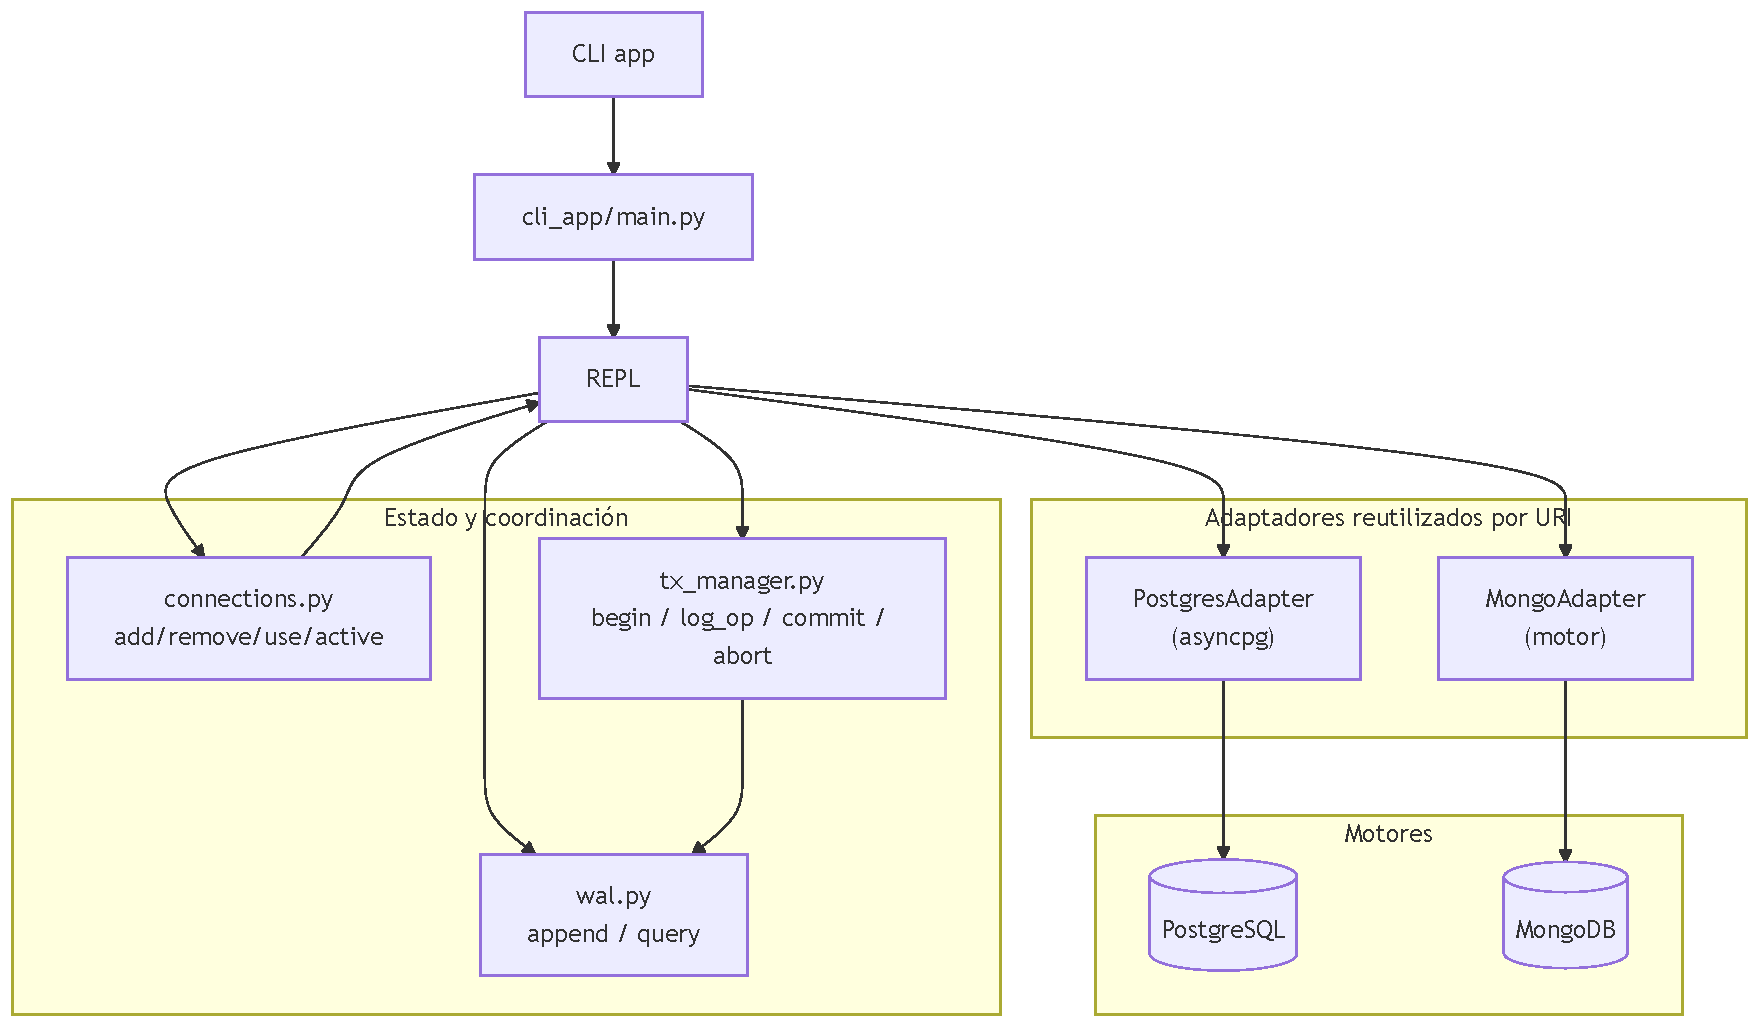
\includegraphics[width=\textwidth]{docs/diagrams/client_architecture.pdf}
  \caption{Diagrama de arquitectura del cliente integrado}
  \label{fig:client-arch}
\end{figure}

\paragraph{Diagrama de protocolos de recuperación}\mbox{}\\

El diagrama de recuperación muestra que el sistema consulta la WAL y, según el protocolo elegido, sigue una de dos rutas: P3 (Undo/No-Redo) o P2 (No-Undo/Redo). En P3, si ocurre una falla antes de confirmar, la recuperación revierte los cambios visibles; en P2, las operaciones confirmadas se rehacen a partir de la bitácora, mientras que las no confirmadas se ignoran. Así se ve de forma clara cómo la bitácora guía la recuperación después de una falla.

\begin{figure}[H]
  \centering
  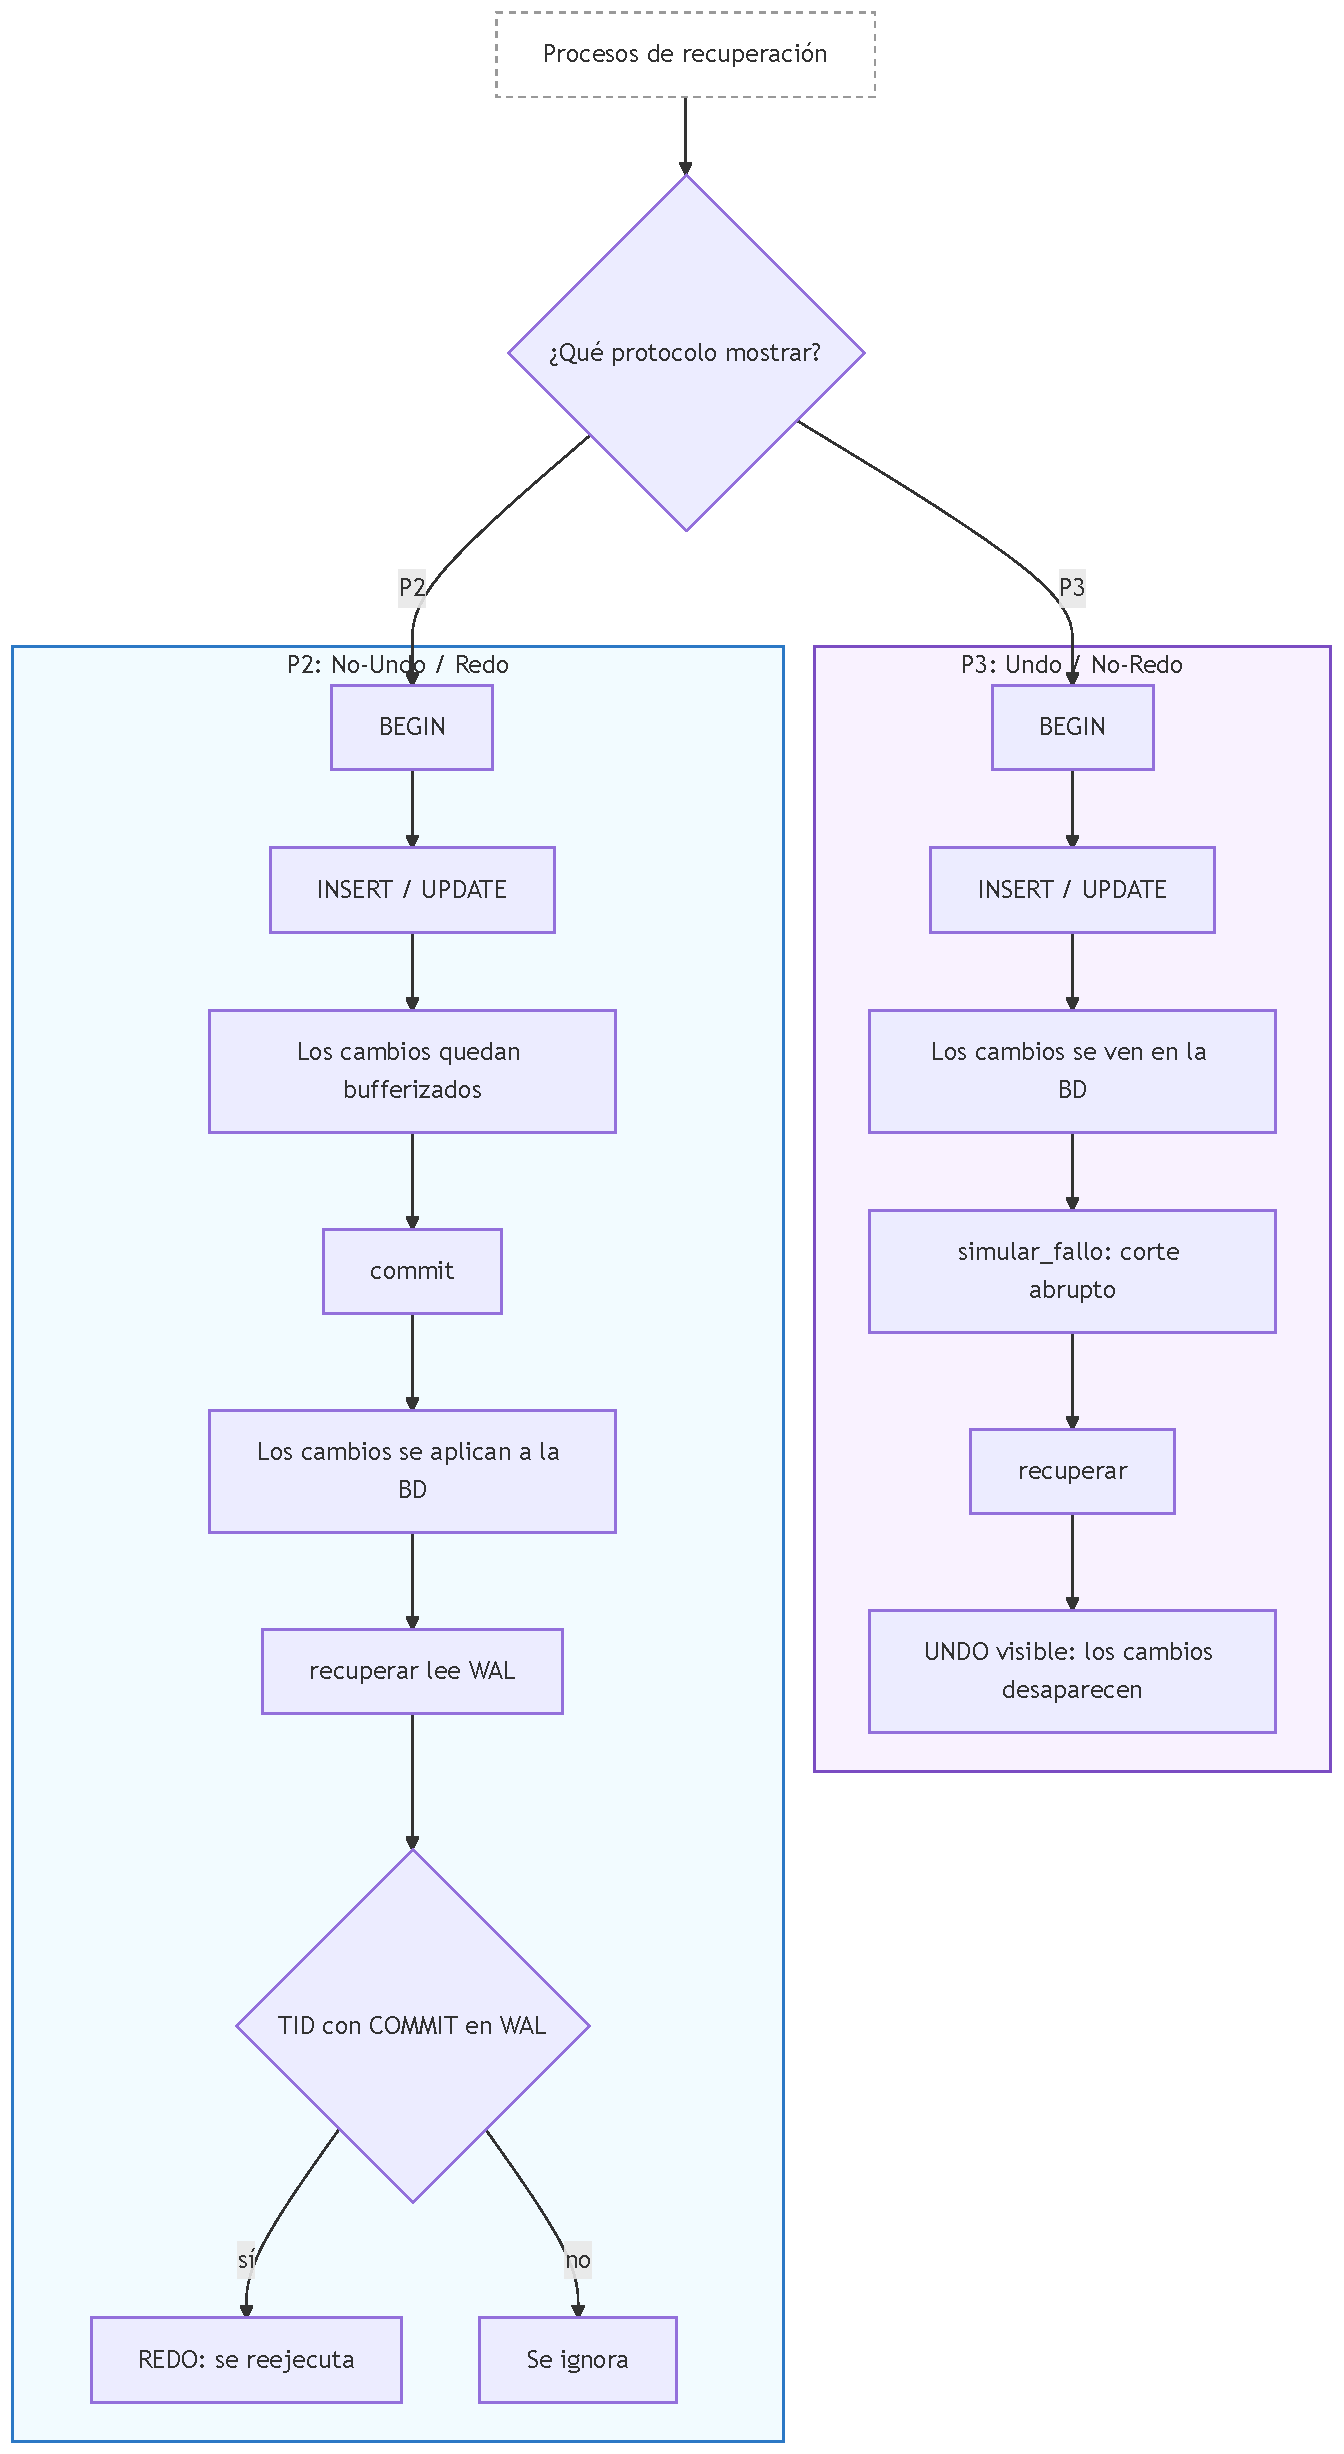
\includegraphics[width=0.85\textwidth]{docs/diagrams/recovery_flow_protocols.pdf}
  \caption{Flujo de los protocolos de recuperación P2 y P3}
  \label{fig:recovery-flow}
\end{figure}

\paragraph{Diagrama de estructura WAL}\mbox{}\\

El diagrama de la WAL muestra cómo cada operación se registra antes de ejecutarse: se crea una entrada, se guarda con \texttt{append(entry)} en formato JSONL y se ordena por LSN. Durante la recuperación, las entradas se recorren en ese orden para aplicar redo o undo según corresponda. Su objetivo es asegurar durabilidad y servir como fuente única de verdad para rehacer o deshacer operaciones de forma determinista.

\begin{figure}[H]
  \centering
  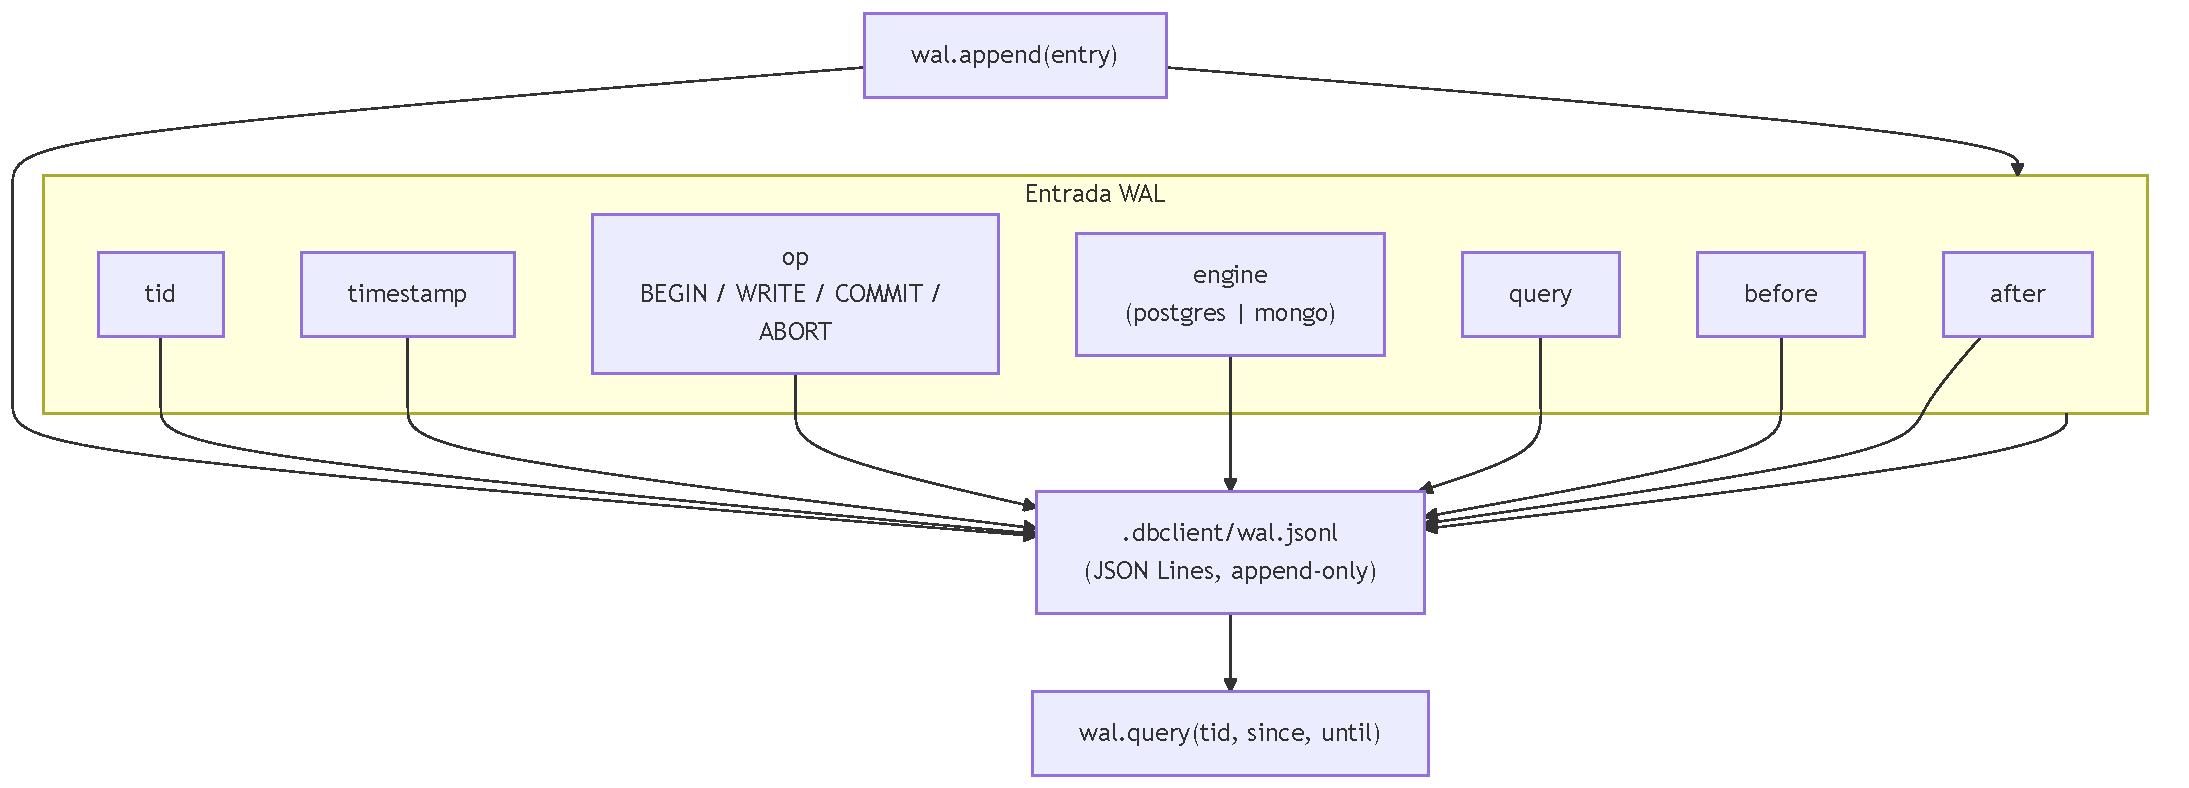
\includegraphics[width=\textwidth]{docs/diagrams/wal_structure.pdf}
  \caption{Estructura de una entrada WAL y operaciones de escritura/consulta}
  \label{fig:wal-structure}
\end{figure}

% ─────────────────────────────────────────────────────────────────────────────
\subsection{Objetivo específico 4: Simulación de fallos en transacciones y aplicación de protocolos de recuperación}
% ─────────────────────────────────────────────────────────────────────────────

El objetivo principal por el cual deben ser implementados los protocolos de recuperación es porque estos son los encargados de materializar los cambios realizados por una transacción en una base de datos y también se encargan de ejecutaras acciones correctas en casos de fallos para devolver la base de datos a un estado consistente. Estos protocolos se diferencian por medio de 2 ejes; escritura (diferida o inmediata) y por las opciones de recuperación necesarias (\textit{UNDO, REDO}, ambas o ninguna).
Estos protocolos de recuperación se apoyan sobre la bitácora de escritura anticipada que se definió en la arquitectura del proyecto, esta funciona mediante un \textit{ Write-Ahead Log, WAL}. Con esto definido podemos entonces definir el funcionamiento e implementación de cada protocolo.

\subsubsection{P1: \textbf{No-Undo / No-Redo}}
Este protocolo utiliza un buffer de memoria sobre el cual se acumulan las opera



% ─────────────────────────────────────────────────────────────────────────────
\section{Conclusiones}
% ─────────────────────────────────────────────────────────────────────────────

% (Esta sección será completada al finalizar los objetivos 3 y 4.)

% ─────────────────────────────────────────────────────────────────────────────
\section*{Referencias}
\addcontentsline{toc}{section}{Referencias}
% ─────────────────────────────────────────────────────────────────────────────

\begin{description}[leftmargin=2em, labelindent=0pt, style=nextline]
  \item[Chavarría, S. A. (2026).] \textit{Especificación del proyecto programado: Cliente
        integrado de motores de bases de datos distribuidas con soporte de consultas,
        bitácora y recuperación ante fallos.} Universidad de Costa Rica, Escuela de
        Ciencias de la Computación e Informática.

  \item[Docker. (2026).] \textit{Docker Compose.} Docker Docs.
        \url{https://docs.docker.com/compose/}

  \item[FastAPI. (2026).] \textit{FastAPI documentation.} Tiangolo.
        \url{https://fastapi.tiangolo.com/}

  \item[MongoDB. (s.f.).] \textit{CRUD operations.} MongoDB Manual.
        \url{https://www.mongodb.com/docs/manual/crud/}

  \item[Pavlo, A. (2022).] \textit{Lecture notes: Logging schemes.} Carnegie Mellon
        University, 15-445/645 Database Systems.
        \url{https://15445.courses.cs.cmu.edu/fall2022/notes/19-logging.pdf}

  \item[PostgreSQL Global Development Group. (2026).] \textit{Write-ahead logging (WAL).}
        PostgreSQL Documentation.
        \url{https://www.postgresql.org/docs/current/wal-intro.html}

  \item[Vue.js. (2026).] \textit{Vue 3 documentation.} The Progressive JavaScript Framework.
        \url{https://vuejs.org/guide/introduction.html}
\end{description}

\end{document}
